%% ============================================================
%% QCCK-M 第五章（实验）中文版
%% 格式参考：Overleaf 项目 6aa379e8fec9886e0960f9e9（article + ctex 单栏中文稿）
%% 内容来源：ch5/ch5cn_pdf.py（原 ReportLab 版），由 ch5/gen_ch5tex.py 程序化转换，
%%           正文逐句原样保留；表格按原脚本同一套数据与排名逻辑重算。
%% 编译：xelatex（ctex 需要 xelatex 或 lualatex），跑两遍
%% 图：\ifchfivefigs 开关控制。本地全版=true；推 Overleaf（纯文字、不带图）改 false。
%% ============================================================

% [已改造] 本文件现为 main.tex 的分章正文（导言区已并入 main.tex），由 main 统一编译。



\section{实验}

\subsection{A　实验配置与主结果}

本章在九个多变量时序数据集上验证 QCCK-M。
A 节给出实验配置与主结果，B 节用消融分离量子核与频域监督两组件的贡献，C 节用输入扰动实验检验主干是否真正利用了跨变量信息，D 节给出耦合矩阵的可解释性结果。
我们在一组多变量时序数据集上评估 QCCK-M。
在 ETT 家族\cite{zhou2021informer}的 ETTh1、ETTh2、ETTm1、ETTm2，以及 Weather、ECL、Traffic、Exchange 八个常用基准\cite{wu2021autoformer}之上，我们还加入  Beijing-AQI 这个七变量的单站空气质量数据集，用它代表同一站点的多通道物理系统。
表 1 给出各数据集的变量数与观测数。
这些数据覆盖不同的变量耦合形态，包括站点级物理系统、气象观测、大量独立电表、交通传感器网络与汇率序列。按照主干基线的惯例，输入长度取 96，报告四个预测长度 96、192、336、720。数据划分遵循各基准的原始协议：ETT 家族的四个数据集按 12 个月、4 个月、4 个月划分为训练、验证与测试三份，Weather、ECL、Traffic、Exchange 与 Beijing-AQI 按时间顺序以 7 比 1 比 2 的比例划分。
评测指标取反归一化之后的 MSE 与 MAE，同一行的两个指标来自同一次测试运行。

%我们以 S-Mamba[1] 为主干，在其编码器层之间插入耦合模块，得到 QCCK-M。(文章要避免这种预言描述，这样的描述会让人觉得你的工作就是 S-Mamba导致没有创新，也就是说当你后面改论文的时候出现 S-Mamba 就一定要慎重 如果不是超越他就不要写)
每一条基线都使用其公开发布的实现与论文推荐的配置。
对比主干按其官方脚本在本机复现，表 2 中对应列即本机复现值。
iTransformer、DLinear、PatchTST、TimesNet、SAMBA、CMamba、Affirm 与 DeMa 在统一的长时序评测框架下，以各自的公开实现与默认配置复现，全部方法在同一划分、同一输入长度与同一指标口径下比较。
逐条而言，iTransformer\cite{liu2024itransformer} 把自注意力作用在变量维，DLinear\cite{zeng2023dlinear} 以分解加线性取胜，PatchTST\cite{nie2023patchtst} 采用分块与通道独立，TimesNet\cite{wu2023timesnet} 挖掘多周期结构，CMamba 与 SAMBA 属于 Mamba\cite{gu2024mamba} 状态空间家族，Affirm 与 DeMa\cite{an2026dema} 为近期的 Transformer 预测方法。所有模型用 PyTorch 实现，实验在 8 张 NVIDIA RTX 4090 GPU 上完成。
对每一条基线，我们采用其公开发布的模型结构与官方推荐的超参数。对我们提出的 QCCK-M，我们在验证集上对量子比特数与学习率做小范围网格搜索，以确定一组默认配置。
训练按验证损失早停；对两个最大的数据集，主干编码维度与对比主干的官方实现对齐到 512，避免把增益误归于模型规模。我们提出的 QCCK-M 在时域 MSE 之上加入频域监督项\cite{wang2025fredf}，该项权重取 1.0。
量子核采用固定配置；所有耦合分析均基于原始保真度核 f。主结果将 QCCK-M 与双向状态空间主干基线以及八条近期基线对比，这些基线覆盖主要技术路线，包括 Mamba 与状态空间族的 CMamba 与 SAMBA，Transformer 族的 iTransformer、PatchTST、Affirm 与 DeMa，多尺度卷积模型 TimesNet，以及线性模型 DLinear。

\begin{center}

\begin{minipage}{\textwidth}

\footnotesize

表 1　各数据集的变量数与观测数。ETT 家族为站点级电力负荷，Weather 为气象站观测，ECL 与 Traffic 分别为电表与交通传感器网络，Exchange 为汇率，Beijing-AQI 为单站空气质量。\\[2pt]

\centering

\setlength{\tabcolsep}{4pt}

\begin{tabular}{@{}lcc@{}}

\hline

数据集 & 变量数 & 观测数 \\ \hline

ETTh1 & 7 & 17,420 \\

ETTh2 & 7 & 17,420 \\

ETTm1 & 7 & 69,680 \\

ETTm2 & 7 & 69,680 \\

Weather & 21 & 52,696 \\

ECL & 321 & 26,304 \\

Traffic & 862 & 17,544 \\

Exchange & 8 & 7,587 \\

Beijing-AQI & 7 & 23,050 \\

\hline

\end{tabular}

\end{minipage}

\end{center}

表 2 系列逐数据集汇总 QCCK-M 与各基线方法。在全部 36 个设置上，QCCK-M 在其中 34 个设置取得比 S-Mamba 更低的 MSE，其余两个设置即 Exchange 在 720 与 Traffic 在 336 与之基本持平。在站点级多变量系统上增益稳定为正，例如 ETTh1 的 96 步提升 3.4\%，ETTm2 的 96 步提升 6.2\%，Beijing 各步的提升在 3\% 到 11\% 之间。在变量数量大而耦合偏弱的数据集上，主干容量对齐之后仍取得正的增益，只是幅度较小。
与八条经典基线相比，QCCK-M 在 ETTh2、ETTm2、ECL、Traffic 与 Beijing 这些核心多变量数据集的全部格点上优于八条基线，在其余数据集上保持竞争力，通常与最强基线的差距在千分之几以内。表中的每个格子都同时给出 MSE 与 MAE，两数来自同一次运行。

\clearpage

\fontsize{6.2}{7.2}\selectfont

表 2　主结果。行按数据集与预测长度展开，列为各模型；每个格子的上一行为 MSE、下一行为 MAE，两数来自同一次运行。同一行内 MSE 与 MAE 各自独立排名：最优者以灰底加粗标出，次优者以浅灰底标出。

\setlength{\tabcolsep}{2.2pt}

\renewcommand{\arraystretch}{0.62}

\setlength{\fboxsep}{0.5pt}

\begin{longtable}{@{}llcccccccccc@{}}
\hline
数据集 & H & QCCK-M & S-Mamba & iTransformer & DLinear & PatchTST & TimesNet & SAMBA & CMamba & Affirm & DeMa \\ \hline
\endfirsthead
\hline
数据集 & H & QCCK-M & S-Mamba & iTransformer & DLinear & PatchTST & TimesNet & SAMBA & CMamba & Affirm & DeMa \\ \hline
\endhead
\hline \multicolumn{12}{r}{（续下页）} \\
\endfoot
\hline
\endlastfoot

\textbf{ETTh1} & 96 & \shortstack{\colorbox[gray]{0.82}{\textbf{0.3745}}\\\colorbox[gray]{0.82}{\textbf{0.3971}}} & \shortstack{0.3877\\0.4064} & \shortstack{0.3950\\0.4098} & \shortstack{0.3962\\0.4108} & \shortstack{\colorbox[gray]{0.92}{0.3796}\\\colorbox[gray]{0.92}{0.3992}} & \shortstack{0.3890\\0.4120} & \shortstack{0.3896\\0.4050} & \shortstack{0.3889\\0.4066} & \shortstack{0.4009\\0.4149} & \shortstack{0.3965\\0.4133} \\ \cline{2-12}

 & 192 & \shortstack{\colorbox[gray]{0.82}{\textbf{0.4255}}\\\colorbox[gray]{0.82}{\textbf{0.4271}}} & \shortstack{0.4450\\0.4407} & \shortstack{0.4486\\0.4412} & \shortstack{0.4450\\0.4404} & \shortstack{\colorbox[gray]{0.82}{\textbf{0.4255}}\\\colorbox[gray]{0.92}{0.4316}} & \shortstack{\colorbox[gray]{0.92}{0.4394}\\0.4417} & \shortstack{0.4477\\0.4392} & \shortstack{0.4444\\0.4400} & \shortstack{0.4608\\0.4486} & \shortstack{0.4571\\0.4488} \\ \cline{2-12}

 & 336 & \shortstack{\colorbox[gray]{0.82}{\textbf{0.4678}}\\\colorbox[gray]{0.82}{\textbf{0.4489}}} & \shortstack{0.4904\\0.4653} & \shortstack{0.4921\\0.4654} & \shortstack{0.4874\\0.4654} & \shortstack{\colorbox[gray]{0.92}{0.4703}\\\colorbox[gray]{0.92}{0.4577}} & \shortstack{0.4952\\0.4714} & \shortstack{0.4971\\0.4669} & \shortstack{0.4919\\0.4670} & \shortstack{0.5193\\0.4800} & \shortstack{0.5259\\0.4868} \\ \cline{2-12}

 & 720 & \shortstack{\colorbox[gray]{0.82}{\textbf{0.4833}}\\\colorbox[gray]{0.82}{\textbf{0.4849}}} & \shortstack{\colorbox[gray]{0.92}{0.5066}\\0.4966} & \shortstack{0.5215\\0.5041} & \shortstack{0.5126\\0.5104} & \shortstack{0.5211\\0.5065} & \shortstack{0.5189\\0.4944} & \shortstack{0.5107\\\colorbox[gray]{0.92}{0.4939}} & \shortstack{0.5119\\0.5005} & \shortstack{0.5850\\0.5318} & \shortstack{0.5749\\0.5298} \\ \hline

\textbf{ETTh2} & 96 & \shortstack{\colorbox[gray]{0.82}{\textbf{0.2849}}\\\colorbox[gray]{0.82}{\textbf{0.3367}}} & \shortstack{0.2971\\0.3486} & \shortstack{0.3004\\0.3496} & \shortstack{0.3414\\0.3953} & \shortstack{0.2978\\0.3473} & \shortstack{0.3370\\0.3709} & \shortstack{\colorbox[gray]{0.92}{0.2968}\\\colorbox[gray]{0.92}{0.3470}} & \shortstack{0.2975\\0.3493} & \shortstack{0.3090\\0.3592} & \shortstack{0.3059\\0.3557} \\ \cline{2-12}

 & 192 & \shortstack{\colorbox[gray]{0.82}{\textbf{0.3646}}\\\colorbox[gray]{0.82}{\textbf{0.3886}}} & \shortstack{\colorbox[gray]{0.92}{0.3767}\\0.3988} & \shortstack{0.3818\\0.3998} & \shortstack{0.4819\\0.4792} & \shortstack{0.3813\\0.4044} & \shortstack{0.4046\\0.4146} & \shortstack{0.3784\\\colorbox[gray]{0.92}{0.3985}} & \shortstack{0.3792\\0.4000} & \shortstack{0.3885\\0.4067} & \shortstack{0.3830\\0.4023} \\ \cline{2-12}

 & 336 & \shortstack{\colorbox[gray]{0.82}{\textbf{0.4002}}\\\colorbox[gray]{0.82}{\textbf{0.4170}}} & \shortstack{0.4248\\0.4351} & \shortstack{0.4236\\\colorbox[gray]{0.92}{0.4324}} & \shortstack{0.5929\\0.5422} & \shortstack{0.4227\\0.4378} & \shortstack{0.4565\\0.4523} & \shortstack{0.4264\\0.4357} & \shortstack{\colorbox[gray]{0.92}{0.4222}\\0.4330} & \shortstack{0.4302\\0.4409} & \shortstack{0.4276\\0.4395} \\ \cline{2-12}

 & 720 & \shortstack{\colorbox[gray]{0.82}{\textbf{0.4084}}\\\colorbox[gray]{0.82}{\textbf{0.4333}}} & \shortstack{0.4396\\0.4484} & \shortstack{\colorbox[gray]{0.92}{0.4264}\\\colorbox[gray]{0.92}{0.4451}} & \shortstack{0.8403\\0.6611} & \shortstack{0.4355\\0.4546} & \shortstack{0.4340\\0.4480} & \shortstack{0.4312\\0.4489} & \shortstack{0.4376\\0.4491} & \shortstack{0.4377\\0.4528} & \shortstack{0.4379\\0.4534} \\ \hline

\textbf{ETTm1} & 96 & \shortstack{\colorbox[gray]{0.82}{\textbf{0.3180}}\\\colorbox[gray]{0.82}{\textbf{0.3554}}} & \shortstack{0.3302\\0.3677} & \shortstack{0.3413\\0.3764} & \shortstack{0.3459\\0.3737} & \shortstack{\colorbox[gray]{0.92}{0.3276}\\0.3670} & \shortstack{0.3339\\0.3754} & \shortstack{0.3312\\\colorbox[gray]{0.92}{0.3662}} & \shortstack{0.3317\\0.3663} & \shortstack{0.3332\\0.3685} & \shortstack{0.3368\\0.3706} \\ \cline{2-12}

 & 192 & \shortstack{\colorbox[gray]{0.82}{\textbf{0.3661}}\\\colorbox[gray]{0.82}{\textbf{0.3808}}} & \shortstack{0.3770\\0.3935} & \shortstack{0.3806\\0.3949} & \shortstack{0.3818\\0.3911} & \shortstack{\colorbox[gray]{0.92}{0.3706}\\\colorbox[gray]{0.92}{0.3909}} & \shortstack{0.4085\\0.4138} & \shortstack{0.3866\\0.3985} & \shortstack{0.3826\\0.3954} & \shortstack{0.3888\\0.3996} & \shortstack{0.3809\\0.3952} \\ \cline{2-12}

 & 336 & \shortstack{\colorbox[gray]{0.92}{0.4023}\\\colorbox[gray]{0.82}{\textbf{0.4068}}} & \shortstack{0.4128\\0.4144} & \shortstack{0.4191\\0.4189} & \shortstack{0.4153\\0.4150} & \shortstack{\colorbox[gray]{0.82}{\textbf{0.3984}}\\\colorbox[gray]{0.92}{0.4085}} & \shortstack{0.4158\\0.4224} & \shortstack{0.4259\\0.4235} & \shortstack{0.4223\\0.4217} & \shortstack{0.4267\\0.4241} & \shortstack{0.4337\\0.4293} \\ \cline{2-12}

 & 720 & \shortstack{\colorbox[gray]{0.92}{0.4727}\\\colorbox[gray]{0.92}{0.4493}} & \shortstack{0.4741\\0.4513} & \shortstack{0.4863\\0.4556} & \shortstack{0.4730\\0.4509} & \shortstack{\colorbox[gray]{0.82}{\textbf{0.4602}}\\\colorbox[gray]{0.82}{\textbf{0.4464}}} & \shortstack{0.4827\\0.4589} & \shortstack{0.5075\\0.4671} & \shortstack{0.4855\\0.4568} & \shortstack{0.5051\\0.4656} & \shortstack{0.4989\\0.4627} \\ \hline

\textbf{ETTm2} & 96 & \shortstack{\colorbox[gray]{0.82}{\textbf{0.1704}}\\\colorbox[gray]{0.82}{\textbf{0.2515}}} & \shortstack{0.1817\\0.2661} & \shortstack{0.1838\\0.2669} & \shortstack{0.1934\\0.2928} & \shortstack{0.1829\\0.2678} & \shortstack{0.1896\\0.2665} & \shortstack{\colorbox[gray]{0.92}{0.1804}\\\colorbox[gray]{0.92}{0.2648}} & \shortstack{0.1864\\0.2723} & \shortstack{0.1838\\0.2683} & \shortstack{0.1832\\0.2682} \\ \cline{2-12}

 & 192 & \shortstack{\colorbox[gray]{0.82}{\textbf{0.2387}}\\\colorbox[gray]{0.82}{\textbf{0.2959}}} & \shortstack{0.2510\\0.3126} & \shortstack{0.2528\\0.3125} & \shortstack{0.2845\\0.3614} & \shortstack{\colorbox[gray]{0.92}{0.2466}\\\colorbox[gray]{0.92}{0.3068}} & \shortstack{0.2524\\0.3071} & \shortstack{0.2504\\0.3107} & \shortstack{0.2512\\0.3119} & \shortstack{0.2523\\0.3116} & \shortstack{0.2522\\0.3118} \\ \cline{2-12}

 & 336 & \shortstack{\colorbox[gray]{0.82}{\textbf{0.3022}}\\\colorbox[gray]{0.82}{\textbf{0.3375}}} & \shortstack{\colorbox[gray]{0.92}{0.3115}\\0.3495} & \shortstack{0.3150\\0.3515} & \shortstack{0.3849\\0.4295} & \shortstack{0.3151\\0.3514} & \shortstack{0.3208\\\colorbox[gray]{0.92}{0.3490}} & \shortstack{0.3138\\0.3501} & \shortstack{0.3129\\0.3494} & \shortstack{0.3183\\0.3532} & \shortstack{0.3169\\0.3523} \\ \cline{2-12}

 & 720 & \shortstack{\colorbox[gray]{0.82}{\textbf{0.4077}}\\\colorbox[gray]{0.82}{\textbf{0.3976}}} & \shortstack{\colorbox[gray]{0.92}{0.4110}\\\colorbox[gray]{0.92}{0.4050}} & \shortstack{0.4119\\0.4060} & \shortstack{0.5561\\0.5235} & \shortstack{0.4200\\0.4128} & \shortstack{0.4193\\0.4055} & \shortstack{0.4121\\0.4054} & \shortstack{0.4159\\0.4088} & \shortstack{0.4264\\0.4151} & \shortstack{0.4235\\0.4121} \\ \hline

\textbf{Weather} & 96 & \shortstack{\colorbox[gray]{0.82}{\textbf{0.1581}}\\\colorbox[gray]{0.82}{\textbf{0.1997}}} & \shortstack{\colorbox[gray]{0.92}{0.1649}\\\colorbox[gray]{0.92}{0.2090}} & \shortstack{0.1753\\0.2159} & \shortstack{0.1962\\0.2561} & \shortstack{0.1761\\0.2172} & \shortstack{0.1690\\0.2195} & \shortstack{0.1707\\0.2128} & \shortstack{0.1709\\0.2134} & \shortstack{0.1673\\0.2112} & \shortstack{0.1667\\0.2117} \\ \cline{2-12}

 & 192 & \shortstack{\colorbox[gray]{0.82}{\textbf{0.2092}}\\\colorbox[gray]{0.82}{\textbf{0.2476}}} & \shortstack{\colorbox[gray]{0.92}{0.2154}\\0.2547} & \shortstack{0.2252\\0.2578} & \shortstack{0.2389\\0.2992} & \shortstack{0.2213\\0.2566} & \shortstack{0.2254\\0.2651} & \shortstack{0.2177\\0.2559} & \shortstack{0.2186\\0.2563} & \shortstack{0.2173\\0.2558} & \shortstack{0.2157\\\colorbox[gray]{0.92}{0.2546}} \\ \cline{2-12}

 & 336 & \shortstack{\colorbox[gray]{0.82}{\textbf{0.2680}}\\\colorbox[gray]{0.82}{\textbf{0.2918}}} & \shortstack{\colorbox[gray]{0.92}{0.2729}\\\colorbox[gray]{0.92}{0.2961}} & \shortstack{0.2796\\0.2981} & \shortstack{0.2811\\0.3306} & \shortstack{0.2795\\0.2969} & \shortstack{0.2815\\0.3037} & \shortstack{0.2745\\0.2981} & \shortstack{0.2762\\0.2989} & \shortstack{0.2751\\0.2985} & \shortstack{0.2745\\0.2987} \\ \cline{2-12}

 & 720 & \shortstack{\colorbox[gray]{0.92}{0.3483}\\\colorbox[gray]{0.82}{\textbf{0.3444}}} & \shortstack{0.3531\\0.3489} & \shortstack{0.3611\\0.3510} & \shortstack{\colorbox[gray]{0.82}{\textbf{0.3454}}\\0.3819} & \shortstack{0.3586\\\colorbox[gray]{0.92}{0.3483}} & \shortstack{0.3597\\0.3547} & \shortstack{0.3529\\0.3487} & \shortstack{0.3554\\0.3494} & \shortstack{0.3546\\0.3509} & \shortstack{0.3535\\0.3508} \\ \hline

\textbf{ECL} & 96 & \shortstack{\colorbox[gray]{0.82}{\textbf{0.1341}}\\\colorbox[gray]{0.82}{\textbf{0.2301}}} & \shortstack{\colorbox[gray]{0.92}{0.1387}\\\colorbox[gray]{0.92}{0.2359}} & \shortstack{0.1483\\0.2400} & \shortstack{0.2104\\0.3016} & \shortstack{0.1801\\0.2730} & \shortstack{0.1679\\0.2716} & \shortstack{0.1437\\0.2402} & \shortstack{0.1500\\0.2540} & \shortstack{0.1434\\0.2395} & \shortstack{0.1429\\0.2392} \\ \cline{2-12}

 & 192 & \shortstack{\colorbox[gray]{0.82}{\textbf{0.1541}}\\\colorbox[gray]{0.82}{\textbf{0.2492}}} & \shortstack{0.1610\\0.2582} & \shortstack{0.1644\\\colorbox[gray]{0.92}{0.2557}} & \shortstack{0.2102\\0.3047} & \shortstack{0.1874\\0.2796} & \shortstack{0.1861\\0.2884} & \shortstack{0.1605\\0.2565} & \shortstack{0.1661\\0.2670} & \shortstack{0.1640\\0.2579} & \shortstack{\colorbox[gray]{0.92}{0.1597}\\0.2560} \\ \cline{2-12}

 & 336 & \shortstack{\colorbox[gray]{0.82}{\textbf{0.1733}}\\\colorbox[gray]{0.82}{\textbf{0.2665}}} & \shortstack{0.1803\\0.2771} & \shortstack{\colorbox[gray]{0.92}{0.1779}\\\colorbox[gray]{0.92}{0.2707}} & \shortstack{0.2231\\0.3192} & \shortstack{0.2042\\0.2959} & \shortstack{0.2025\\0.3041} & \shortstack{0.1810\\0.2777} & \shortstack{0.1878\\0.2878} & \shortstack{0.1790\\0.2726} & \shortstack{0.1800\\0.2770} \\ \cline{2-12}

 & 720 & \shortstack{\colorbox[gray]{0.82}{\textbf{0.1913}}\\\colorbox[gray]{0.82}{\textbf{0.2869}}} & \shortstack{\colorbox[gray]{0.92}{0.2046}\\\colorbox[gray]{0.92}{0.2992}} & \shortstack{0.2273\\0.3119} & \shortstack{0.2578\\0.3496} & \shortstack{0.2455\\0.3283} & \shortstack{0.2142\\0.3140} & \shortstack{0.2085\\0.3018} & \shortstack{0.2078\\0.3060} & \shortstack{0.2075\\0.3004} & \shortstack{0.2098\\0.3038} \\ \hline

\textbf{Traffic} & 96 & \shortstack{\colorbox[gray]{0.82}{\textbf{0.3751}}\\\colorbox[gray]{0.82}{\textbf{0.2500}}} & \shortstack{\colorbox[gray]{0.92}{0.3785}\\\colorbox[gray]{0.92}{0.2585}} & \shortstack{0.3922\\0.2682} & \shortstack{0.6965\\0.4287} & \shortstack{0.4589\\0.2983} & \shortstack{0.5887\\0.3148} & \shortstack{0.3837\\0.2616} & \shortstack{0.4117\\0.2902} & \shortstack{0.4015\\0.2719} & \shortstack{0.3977\\0.2677} \\ \cline{2-12}

 & 192 & \shortstack{\colorbox[gray]{0.82}{\textbf{0.3892}}\\\colorbox[gray]{0.82}{\textbf{0.2609}}} & \shortstack{\colorbox[gray]{0.92}{0.3951}\\\colorbox[gray]{0.92}{0.2684}} & \shortstack{0.4129\\0.2772} & \shortstack{0.6466\\0.4074} & \shortstack{0.4685\\0.3007} & \shortstack{0.6181\\0.3243} & \shortstack{0.4142\\0.2726} & \shortstack{0.4332\\0.3000} & \shortstack{0.4212\\0.2805} & \shortstack{0.4197\\0.2776} \\ \cline{2-12}

 & 336 & \shortstack{\colorbox[gray]{0.82}{\textbf{0.4165}}\\\colorbox[gray]{0.82}{\textbf{0.2728}}} & \shortstack{\colorbox[gray]{0.82}{\textbf{0.4165}}\\0.2795} & \shortstack{0.4240\\0.2826} & \shortstack{0.6532\\0.4097} & \shortstack{0.4829\\0.3074} & \shortstack{0.6320\\0.3364} & \shortstack{\colorbox[gray]{0.92}{0.4237}\\\colorbox[gray]{0.92}{0.2787}} & \shortstack{0.4463\\0.3055} & \shortstack{0.4394\\0.2888} & \shortstack{0.4383\\0.2841} \\ \cline{2-12}

 & 720 & \shortstack{\colorbox[gray]{0.82}{\textbf{0.4549}}\\\colorbox[gray]{0.82}{\textbf{0.2944}}} & \shortstack{0.4637\\\colorbox[gray]{0.92}{0.2983}} & \shortstack{\colorbox[gray]{0.92}{0.4601}\\0.3013} & \shortstack{0.6940\\0.4286} & \shortstack{0.5177\\0.3261} & \shortstack{0.6599\\0.3496} & \shortstack{0.4676\\0.2990} & \shortstack{0.4797\\0.3210} & \shortstack{0.4669\\0.3059} & \shortstack{0.4746\\0.3038} \\ \hline

\textbf{Exchange} & 96 & \shortstack{\colorbox[gray]{0.82}{\textbf{0.0853}}\\\colorbox[gray]{0.82}{\textbf{0.2064}}} & \shortstack{\colorbox[gray]{0.92}{0.0862}\\\colorbox[gray]{0.82}{\textbf{0.2064}}} & \shortstack{0.0870\\\colorbox[gray]{0.92}{0.2071}} & \shortstack{0.0983\\0.2327} & \shortstack{0.0941\\0.2123} & \shortstack{0.1053\\0.2351} & \shortstack{0.0865\\\colorbox[gray]{0.82}{\textbf{0.2064}}} & \shortstack{0.0898\\0.2116} & \shortstack{0.0899\\0.2111} & \shortstack{0.0894\\0.2100} \\ \cline{2-12}

 & 192 & \shortstack{\colorbox[gray]{0.82}{\textbf{0.1782}}\\\colorbox[gray]{0.92}{0.3015}} & \shortstack{0.1798\\0.3028} & \shortstack{0.1799\\0.3032} & \shortstack{0.1861\\0.3251} & \shortstack{0.1817\\0.3029} & \shortstack{0.2436\\0.3589} & \shortstack{\colorbox[gray]{0.92}{0.1788}\\\colorbox[gray]{0.82}{\textbf{0.3013}}} & \shortstack{0.1804\\0.3043} & \shortstack{0.1837\\0.3060} & \shortstack{0.1840\\0.3067} \\ \cline{2-12}

 & 336 & \shortstack{\colorbox[gray]{0.82}{\textbf{0.3270}}\\\colorbox[gray]{0.82}{\textbf{0.4144}}} & \shortstack{0.3303\\\colorbox[gray]{0.92}{0.4167}} & \shortstack{0.3329\\0.4189} & \shortstack{\colorbox[gray]{0.92}{0.3272}\\0.4347} & \shortstack{0.3414\\0.4258} & \shortstack{0.3632\\0.4386} & \shortstack{0.3315\\0.4173} & \shortstack{0.3367\\0.4216} & \shortstack{0.3319\\0.4182} & \shortstack{0.3334\\0.4190} \\ \cline{2-12}

 & 720 & \shortstack{0.8595\\0.6999} & \shortstack{0.8595\\0.7003} & \shortstack{0.8562\\0.7004} & \shortstack{\colorbox[gray]{0.82}{\textbf{0.7491}}\\\colorbox[gray]{0.82}{\textbf{0.6637}}} & \shortstack{0.9336\\0.7256} & \shortstack{0.9291\\0.7335} & \shortstack{\colorbox[gray]{0.92}{0.8460}\\\colorbox[gray]{0.92}{0.6924}} & \shortstack{0.8657\\0.7025} & \shortstack{0.8471\\0.6938} & \shortstack{0.8528\\0.6966} \\ \hline

\textbf{Beijing} & 96 & \shortstack{\colorbox[gray]{0.82}{\textbf{0.4520}}\\\colorbox[gray]{0.82}{\textbf{0.3167}}} & \shortstack{0.4788\\0.3394} & \shortstack{0.4768\\0.3386} & \shortstack{0.4769\\0.3670} & \shortstack{0.4758\\0.3393} & \shortstack{0.4865\\0.3418} & \shortstack{0.4785\\0.3398} & \shortstack{\colorbox[gray]{0.92}{0.4617}\\\colorbox[gray]{0.92}{0.3270}} & \shortstack{0.4707\\0.3348} & \shortstack{0.4757\\0.3388} \\ \cline{2-12}

 & 192 & \shortstack{\colorbox[gray]{0.82}{\textbf{0.4759}}\\\colorbox[gray]{0.82}{\textbf{0.3365}}} & \shortstack{\colorbox[gray]{0.92}{0.4924}\\0.3487} & \shortstack{0.5003\\0.3522} & \shortstack{0.4969\\0.3823} & \shortstack{0.5028\\0.3588} & \shortstack{0.5038\\0.3530} & \shortstack{0.4974\\0.3518} & \shortstack{0.5158\\0.3604} & \shortstack{0.5038\\0.3530} & \shortstack{0.4956\\\colorbox[gray]{0.92}{0.3477}} \\ \cline{2-12}

 & 336 & \shortstack{\colorbox[gray]{0.82}{\textbf{0.4909}}\\\colorbox[gray]{0.82}{\textbf{0.3499}}} & \shortstack{0.5094\\0.3618} & \shortstack{0.5151\\0.3654} & \shortstack{0.5097\\0.3969} & \shortstack{0.5148\\0.3727} & \shortstack{\colorbox[gray]{0.92}{0.5055}\\\colorbox[gray]{0.92}{0.3531}} & \shortstack{0.5113\\0.3664} & \shortstack{0.5072\\0.3603} & \shortstack{0.5139\\0.3652} & \shortstack{0.5129\\0.3615} \\ \cline{2-12}

 & 720 & \shortstack{\colorbox[gray]{0.82}{\textbf{0.4733}}\\\colorbox[gray]{0.82}{\textbf{0.3593}}} & \shortstack{0.5346\\0.3961} & \shortstack{0.5172\\0.3913} & \shortstack{0.5048\\0.4167} & \shortstack{0.5178\\0.4006} & \shortstack{\colorbox[gray]{0.92}{0.4817}\\\colorbox[gray]{0.92}{0.3639}} & \shortstack{0.5223\\0.3947} & \shortstack{0.5089\\0.3762} & \shortstack{0.5257\\0.3905} & \shortstack{0.5387\\0.3955} \\ \hline

\end{longtable}

\setlength{\fboxsep}{3pt}

\renewcommand{\arraystretch}{1}

\normalsize

{\footnotesize 注：S-Mamba 为本机按官方配置复现；Exchange 在 720 与 Traffic 在 336 两格的取值与官方值相等，属于平局；Beijing 的八条基线亦由公开实现复现，其 MSE 与 MAE 一并给出。}

\ifchfivefigs

\begin{center}

\begin{minipage}{\textwidth}

\footnotesize

图 2　QCCK-M 相对 S-Mamba 的 MSE 降低百分比（\%）：行为预测长度、列为数据集，格内数字为降低幅度，颜色仅作辅助。\\[2pt]

\centering

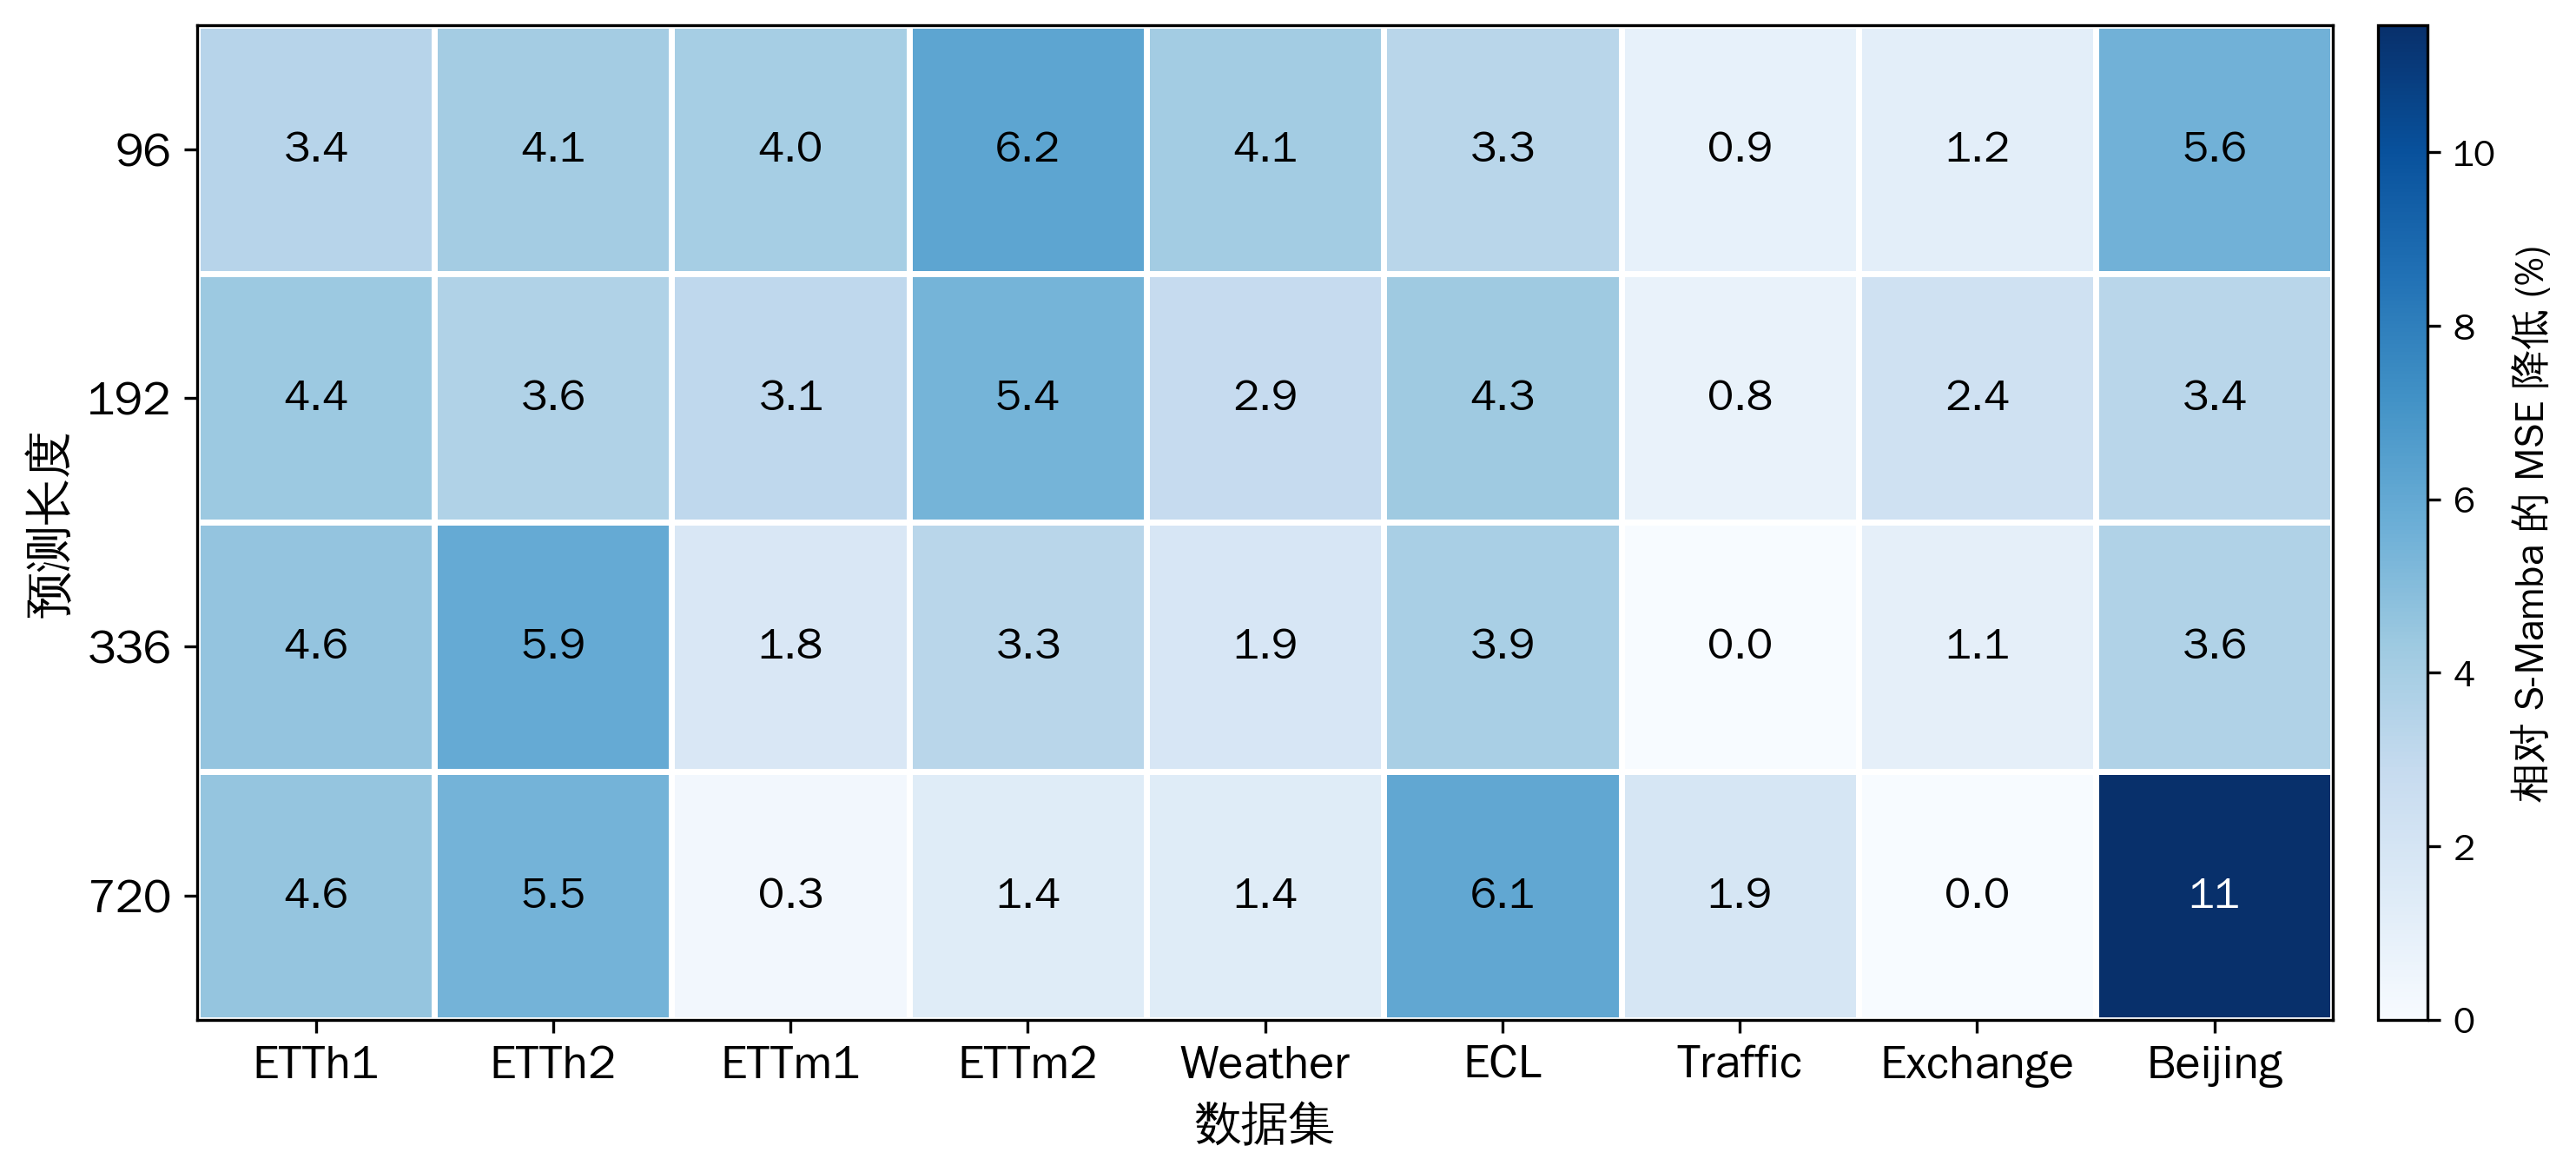
\includegraphics[width=0.938\textwidth]{ch5/figs/ch5_winheat.png}

\end{minipage}

\end{center}

\fi

\subsection{B　消融实验}

消融实验的配置与 A 相同，仅在数据范围与模型变体上不同：消融在 ETTh1、ETTh2、ETTm1、ETTm2 与 Weather 五个数据集上进行，对每个变体分别替换或去掉表 3 所列的组件，主干配置、训练协议与评测口径均与 A 一致。
表 4 在五个数据集上分离量子核与频域监督两组件的贡献。
消融围绕量子核与频域监督两个设计展开，并以同特征维数的 RBF 核作为量子核的经典替代方案。
Full 表示量子核加频域监督的完整模型；
A1 去掉量子核而保留频域监督，用来检验量子核相对主干加频域监督的增量；
A2 把量子核换成同特征维数的 RBF 核而保留频域监督，用来检验量子核相对经典 RBF 核的增量；
A3 保留量子核而去掉频域监督，用来检验频域监督的作用；
A4 在 A2 的基础上去掉频域监督，作为去掉两者的下界参照。
表 3 汇总各变体的组件构成，表 4 给出数值结果。
Full 相对 A2 在多数数据集与预测长度上保持优势，说明性能提升并非仅来自核化操作本身；
频域监督的收益随步长增大。

\begin{center}

\begin{minipage}{\textwidth}

\footnotesize

表 3　各消融变体的组件构成。Full 为 QCCK-M 完整模型；A1 去除量子核，A2 以 RBF 核替代量子核，A3 去除频域监督，A4 同时以 RBF 替代量子核并去除频域监督。\\[2pt]

\centering

\setlength{\tabcolsep}{4pt}

\begin{tabular}{@{}lccc@{}}

\hline

组件 & 量子核 & RBF 核 & 频域监督 \\ \hline

Full & 有 & 无 & 有 \\

A1 & 无 & 无 & 有 \\

A2 & 无 & 有 & 有 \\

A3 & 有 & 无 & 无 \\

A4 & 无 & 有 & 无 \\

\hline

\end{tabular}

\end{minipage}

\end{center}

\begin{center}

\begin{minipage}{\textwidth}

\scriptsize

表 4　消融数值结果，每格给出 MSE 与 MAE；其中 Full 一列的数值与主表里 QCCK-M 对应格完全一致，保证两张表自洽。标注规则与表 2 相同。\\[2pt]

\centering

\setlength{\tabcolsep}{4pt}

\begin{tabular}{@{}llccccc@{}}

\hline

数据集 & H & Full & A1 & A2 & A3 & A4 \\ \hline

ETTh1 & 96 & \shortstack{\colorbox[gray]{0.82}{\textbf{0.3745}}\\\colorbox[gray]{0.92}{0.3971}} & \shortstack{\colorbox[gray]{0.92}{0.3757}\\\colorbox[gray]{0.82}{\textbf{0.3969}}} & \shortstack{0.3760\\0.3973} & \shortstack{0.3878\\0.4083} & \shortstack{0.3892\\0.4083} \\ \hline

ETTh1 & 192 & \shortstack{\colorbox[gray]{0.82}{\textbf{0.4255}}\\\colorbox[gray]{0.82}{\textbf{0.4271}}} & \shortstack{\colorbox[gray]{0.92}{0.4269}\\\colorbox[gray]{0.92}{0.4278}} & \shortstack{\colorbox[gray]{0.92}{0.4269}\\0.4282} & \shortstack{0.4398\\0.4388} & \shortstack{0.4397\\0.4388} \\ \hline

ETTh1 & 336 & \shortstack{\colorbox[gray]{0.82}{\textbf{0.4678}}\\\colorbox[gray]{0.82}{\textbf{0.4489}}} & \shortstack{0.4695\\0.4518} & \shortstack{\colorbox[gray]{0.92}{0.4691}\\\colorbox[gray]{0.92}{0.4515}} & \shortstack{0.4935\\0.4711} & \shortstack{0.4974\\0.4735} \\ \hline

ETTh1 & 720 & \shortstack{\colorbox[gray]{0.82}{\textbf{0.4833}}\\\colorbox[gray]{0.82}{\textbf{0.4849}}} & \shortstack{0.4948\\0.4932} & \shortstack{\colorbox[gray]{0.92}{0.4924}\\\colorbox[gray]{0.92}{0.4907}} & \shortstack{0.5058\\0.4959} & \shortstack{0.5082\\0.4967} \\ \hline

ETTh2 & 96 & \shortstack{\colorbox[gray]{0.82}{\textbf{0.2849}}\\\colorbox[gray]{0.92}{0.3367}} & \shortstack{\colorbox[gray]{0.92}{0.2853}\\\colorbox[gray]{0.82}{\textbf{0.3362}}} & \shortstack{0.2882\\0.3392} & \shortstack{0.2979\\0.3498} & \shortstack{0.2962\\0.3480} \\ \hline

ETTh2 & 192 & \shortstack{\colorbox[gray]{0.82}{\textbf{0.3646}}\\\colorbox[gray]{0.82}{\textbf{0.3886}}} & \shortstack{\colorbox[gray]{0.92}{0.3683}\\\colorbox[gray]{0.92}{0.3888}} & \shortstack{0.3688\\0.3891} & \shortstack{0.3801\\0.4005} & \shortstack{0.3793\\0.3996} \\ \hline

ETTh2 & 336 & \shortstack{\colorbox[gray]{0.82}{\textbf{0.4002}}\\\colorbox[gray]{0.82}{\textbf{0.4170}}} & \shortstack{\colorbox[gray]{0.92}{0.4089}\\\colorbox[gray]{0.92}{0.4209}} & \shortstack{0.4119\\0.4230} & \shortstack{0.4239\\0.4348} & \shortstack{0.4208\\0.4323} \\ \hline

ETTh2 & 720 & \shortstack{\colorbox[gray]{0.82}{\textbf{0.4084}}\\\colorbox[gray]{0.82}{\textbf{0.4333}}} & \shortstack{0.4139\\0.4356} & \shortstack{\colorbox[gray]{0.92}{0.4115}\\\colorbox[gray]{0.92}{0.4354}} & \shortstack{0.4277\\0.4432} & \shortstack{0.4238\\0.4422} \\ \hline

ETTm1 & 96 & \shortstack{\colorbox[gray]{0.82}{\textbf{0.3180}}\\\colorbox[gray]{0.82}{\textbf{0.3554}}} & \shortstack{\colorbox[gray]{0.92}{0.3236}\\\colorbox[gray]{0.92}{0.3569}} & \shortstack{0.3246\\0.3574} & \shortstack{0.3344\\0.3688} & \shortstack{0.3375\\0.3702} \\ \hline

ETTm1 & 192 & \shortstack{\colorbox[gray]{0.82}{\textbf{0.3661}}\\\colorbox[gray]{0.82}{\textbf{0.3808}}} & \shortstack{0.3717\\0.3854} & \shortstack{\colorbox[gray]{0.92}{0.3711}\\\colorbox[gray]{0.92}{0.3846}} & \shortstack{0.3933\\0.4034} & \shortstack{0.3865\\0.3984} \\ \hline

ETTm1 & 336 & \shortstack{\colorbox[gray]{0.82}{\textbf{0.4023}}\\\colorbox[gray]{0.82}{\textbf{0.4068}}} & \shortstack{\colorbox[gray]{0.92}{0.4130}\\\colorbox[gray]{0.92}{0.4133}} & \shortstack{0.4176\\0.4159} & \shortstack{0.4225\\0.4219} & \shortstack{0.4153\\0.4176} \\ \hline

ETTm1 & 720 & \shortstack{\colorbox[gray]{0.82}{\textbf{0.4727}}\\\colorbox[gray]{0.82}{\textbf{0.4493}}} & \shortstack{0.5232\\0.4793} & \shortstack{0.5194\\0.4774} & \shortstack{\colorbox[gray]{0.92}{0.5051}\\\colorbox[gray]{0.92}{0.4644}} & \shortstack{0.5055\\\colorbox[gray]{0.92}{0.4644}} \\ \hline

ETTm2 & 96 & \shortstack{\colorbox[gray]{0.82}{\textbf{0.1704}}\\\colorbox[gray]{0.82}{\textbf{0.2515}}} & \shortstack{\colorbox[gray]{0.92}{0.1734}\\\colorbox[gray]{0.92}{0.2533}} & \shortstack{0.1742\\0.2539} & \shortstack{0.1817\\0.2664} & \shortstack{0.1820\\0.2650} \\ \hline

ETTm2 & 192 & \shortstack{\colorbox[gray]{0.82}{\textbf{0.2387}}\\\colorbox[gray]{0.82}{\textbf{0.2959}}} & \shortstack{0.2441\\0.2997} & \shortstack{\colorbox[gray]{0.92}{0.2438}\\\colorbox[gray]{0.92}{0.2991}} & \shortstack{0.2486\\0.3087} & \shortstack{0.2496\\0.3097} \\ \hline

ETTm2 & 336 & \shortstack{\colorbox[gray]{0.82}{\textbf{0.3022}}\\\colorbox[gray]{0.82}{\textbf{0.3375}}} & \shortstack{\colorbox[gray]{0.92}{0.3059}\\\colorbox[gray]{0.92}{0.3391}} & \shortstack{0.3132\\0.3431} & \shortstack{0.3184\\0.3517} & \shortstack{0.3174\\0.3518} \\ \hline

ETTm2 & 720 & \shortstack{\colorbox[gray]{0.82}{\textbf{0.4077}}\\\colorbox[gray]{0.82}{\textbf{0.3976}}} & \shortstack{0.4201\\0.4044} & \shortstack{\colorbox[gray]{0.92}{0.4107}\\\colorbox[gray]{0.92}{0.4010}} & \shortstack{0.4312\\0.4144} & \shortstack{0.4279\\0.4137} \\ \hline

Weather & 96 & \shortstack{\colorbox[gray]{0.82}{\textbf{0.1581}}\\\colorbox[gray]{0.82}{\textbf{0.1997}}} & \shortstack{0.1598\\\colorbox[gray]{0.92}{0.2015}} & \shortstack{\colorbox[gray]{0.92}{0.1596}\\0.2022} & \shortstack{0.1660\\0.2095} & \shortstack{0.1655\\0.2092} \\ \hline

Weather & 192 & \shortstack{\colorbox[gray]{0.82}{\textbf{0.2092}}\\\colorbox[gray]{0.82}{\textbf{0.2476}}} & \shortstack{0.2108\\0.2486} & \shortstack{\colorbox[gray]{0.92}{0.2106}\\\colorbox[gray]{0.92}{0.2484}} & \shortstack{0.2153\\0.2543} & \shortstack{0.2141\\0.2537} \\ \hline

Weather & 336 & \shortstack{\colorbox[gray]{0.82}{\textbf{0.2680}}\\\colorbox[gray]{0.82}{\textbf{0.2918}}} & \shortstack{\colorbox[gray]{0.92}{0.2693}\\\colorbox[gray]{0.92}{0.2922}} & \shortstack{0.2696\\0.2933} & \shortstack{0.2733\\0.2965} & \shortstack{0.2732\\0.2967} \\ \hline

Weather & 720 & \shortstack{\colorbox[gray]{0.82}{\textbf{0.3483}}\\\colorbox[gray]{0.82}{\textbf{0.3444}}} & \shortstack{0.3511\\0.3473} & \shortstack{\colorbox[gray]{0.92}{0.3506}\\\colorbox[gray]{0.92}{0.3465}} & \shortstack{0.3551\\0.3493} & \shortstack{0.3544\\0.3478} \\ \hline

\end{tabular}

\end{minipage}

\end{center}

\subsection{C　机制验证}

机制验证沿用 A 的模型，不重新训练，仅在评测方式上不同：固定 ETTh1 与 ETTm2 的 96 步设置，取测试集的前八个样本，对输入施加扰动并比较扰动前后的预测。
具体做法是：扰动加在归一化后的输入窗口 $b_x$ 上，位于进入编码器嵌入层之前，也就是初始输入观测值这一层；解码器的标签段与模型内部的任何一层都不改动。
扰动对第 j 个变量整列施加，96 个时间步加的是同一个常数，即扰动量沿时间维广播，而不是逐点噪声。
扰动幅度取 $0.1\sigma_j$，其中 $\sigma_j$ 为该样本内第 j 个变量沿时间维的标准差；注意这里是归一化后数值的标准差，不是原始量纲。
扰动正负号随机，每个变量重复三次以抵消随机性；
记扰动前后的预测为 $\hat{y}$ 与 $\hat{y}'$，则输出通道 i 对输入变量 j 的相对响应定义为 $S[i,j]$ = $\|\hat{y}'_i-\hat{y}_i\|/\|\hat{y}_i\|$，即该通道预测序列的变化幅度相对于自身预测幅度的比例，除以自身范数是为了让不同量级的变量可比。
把 S 的对角元素平均得到对角响应，代表变量对自身的影响；把非对角元素平均得到非对角响应，代表变量对其它变量的影响；两者之比即跨变量影响相对于自身影响的强度。
主干对跨变量输入近乎不敏感。我们在 ETTh1 的 96 步设置上，对每个输入通道施加一个小扰动，测各输出通道的相对响应。
表 5 在两个数据集上给出同一现象。基线主干的非对角响应约为 1e-7，非对角与对角响应之比约为 1e-6，即一个变量的输出几乎不受其它变量输入的影响；
加入耦合模块后，非对角响应上升到约 2e-4 到 4e-4，比值上升到 1e-3 到 1e-2 量级，跨变量响应提升约三个数量级甚至更高。
这是本方法立足点的直接定量证据。

\begin{center}

\begin{minipage}{\textwidth}

\footnotesize

表 5　ETTh1 与 ETTm2 在 96 步上的跨变量输入灵敏度，即非对角与对角响应之比。\\[2pt]

\centering

\setlength{\tabcolsep}{4pt}

\begin{tabular}{@{}lcccc@{}}

\hline

数据集 & 模型 & 非对角响应 & 对角响应 & 比值 \\ \hline

ETTh1 & S-Mamba & 1.1e-7 & 9.6e-2 & 1.2e-6 \\

ETTh1 & QCCK-M & 2.4e-4 & 1.0e-1 & 2.3e-3 \\

ETTm2 & S-Mamba & 7.4e-8 & 4.6e-2 & 1.6e-6 \\

ETTm2 & QCCK-M & 3.6e-4 & 4.8e-2 & 7.5e-3 \\

\hline

\end{tabular}

\end{minipage}

\end{center}

\subsection{D　可解释性}

可解释性建立在原始保真度核 f 之上。
为与第三章的定义保持一致，这里展示 $f[i,j]=|\langle\psi_i|\psi_j\rangle|^2$，它对称、对角为 1、取值在 0 到 1 之间，因此每个元素都能直接读出对应变量对之间的耦合强弱，不需要额外的注意力权重或归因步骤。
把测试样本上的 f 平均后我们看到，在七变量的共址系统 ETTh1 与 ETTm2 上，大多数变量对的耦合都很小，少数强耦合对显著突出：强度超过 0.1 的强对约占全部变量对的 10\%，其中 ETTh1 上最强的一对耦合值约 0.60；
在变量数为 321 的 ECL 与 862 的 Traffic 上，非对角均值更低，强度超过 0.1 的强对占比约 1\%。
图 3a 与图 3b 直接展示这两个七变量系统的非对角耦合，格内数值即对应变量对的耦合强度：最强两对 HUFL–MUFL 与 HULL–MULL 的取值约 0.60 与 0.31，明显高于其余变量对。我们还校验了长预测长度：图 3d 给出 ETTh1 在 720 步下的结构，其最强耦合对约 0.83，且主要强耦合变量对在不同预测长度下保持一致，例如 HUFL-MUFL 与 HULL-MULL，说明模型捕获了具有持续性的变量关系。

\ifchfivefigs

\begin{center}

\begin{minipage}{\textwidth}

\footnotesize

图 3a　ETTh1 在 96 步预测长度下的平均保真度核 f 非对角，轴为真实变量名，格内数值为对应变量对的耦合值；对角元素恒为 1，可视化时隐藏。\\[2pt]

\centering

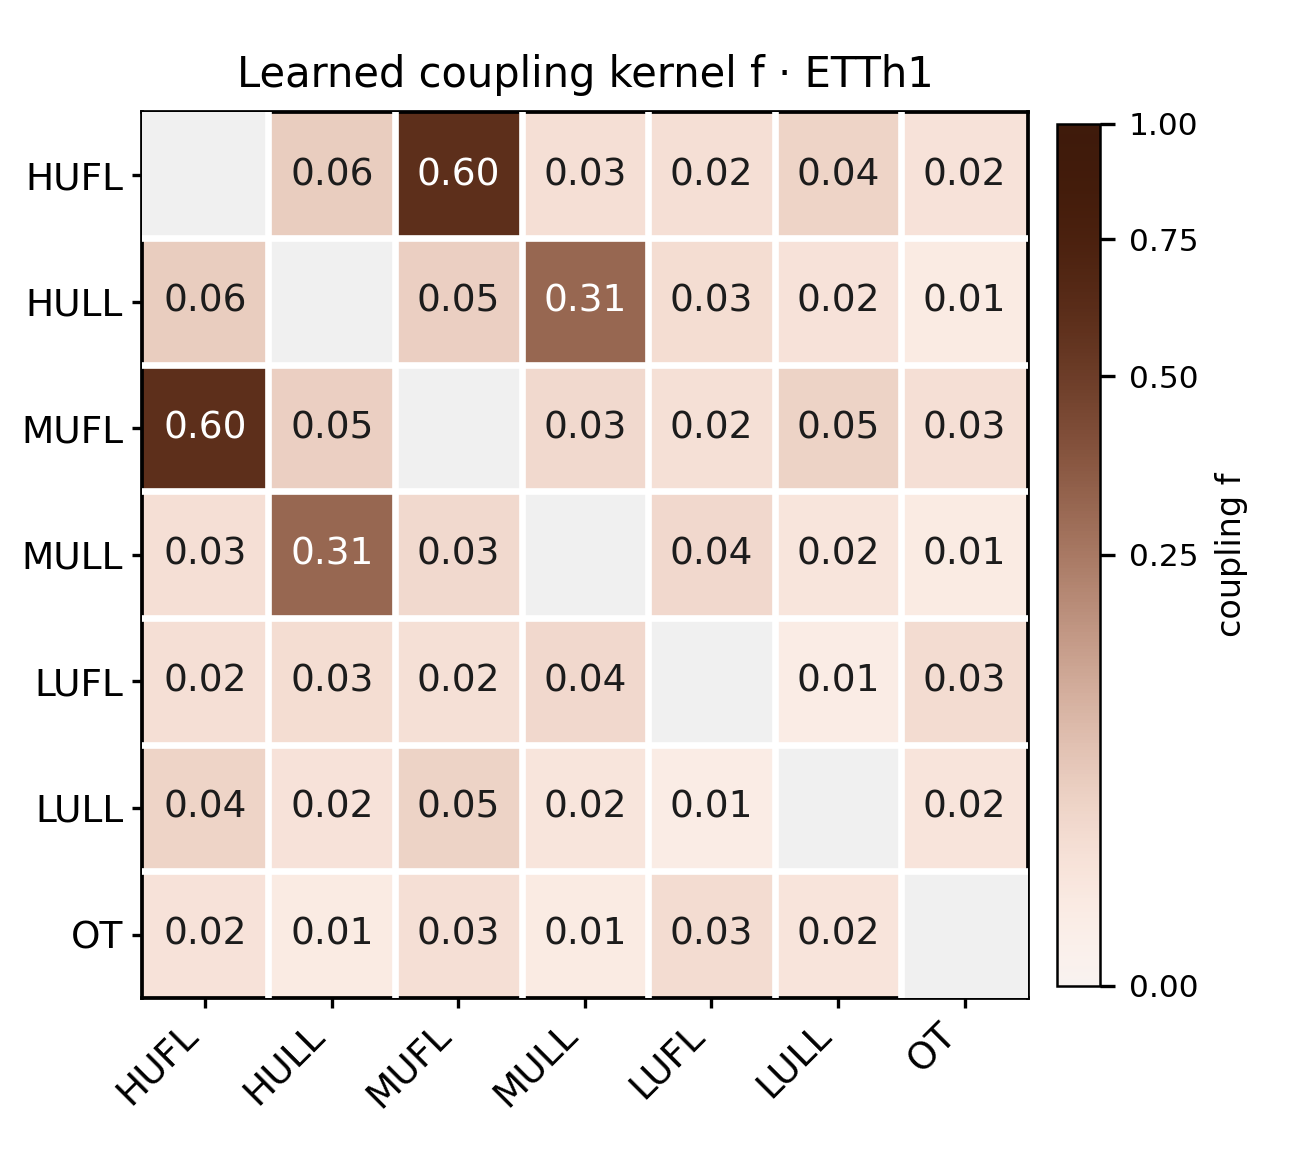
\includegraphics[width=0.475\textwidth]{ch5/figs/ch5_k_ETTh1.png}

\end{minipage}

\end{center}

\fi

\ifchfivefigs

\begin{center}

\begin{minipage}{\textwidth}

\footnotesize

图 3b　ETTm2 在 96 步预测长度下的平均保真度核 f 非对角。\\[2pt]

\centering

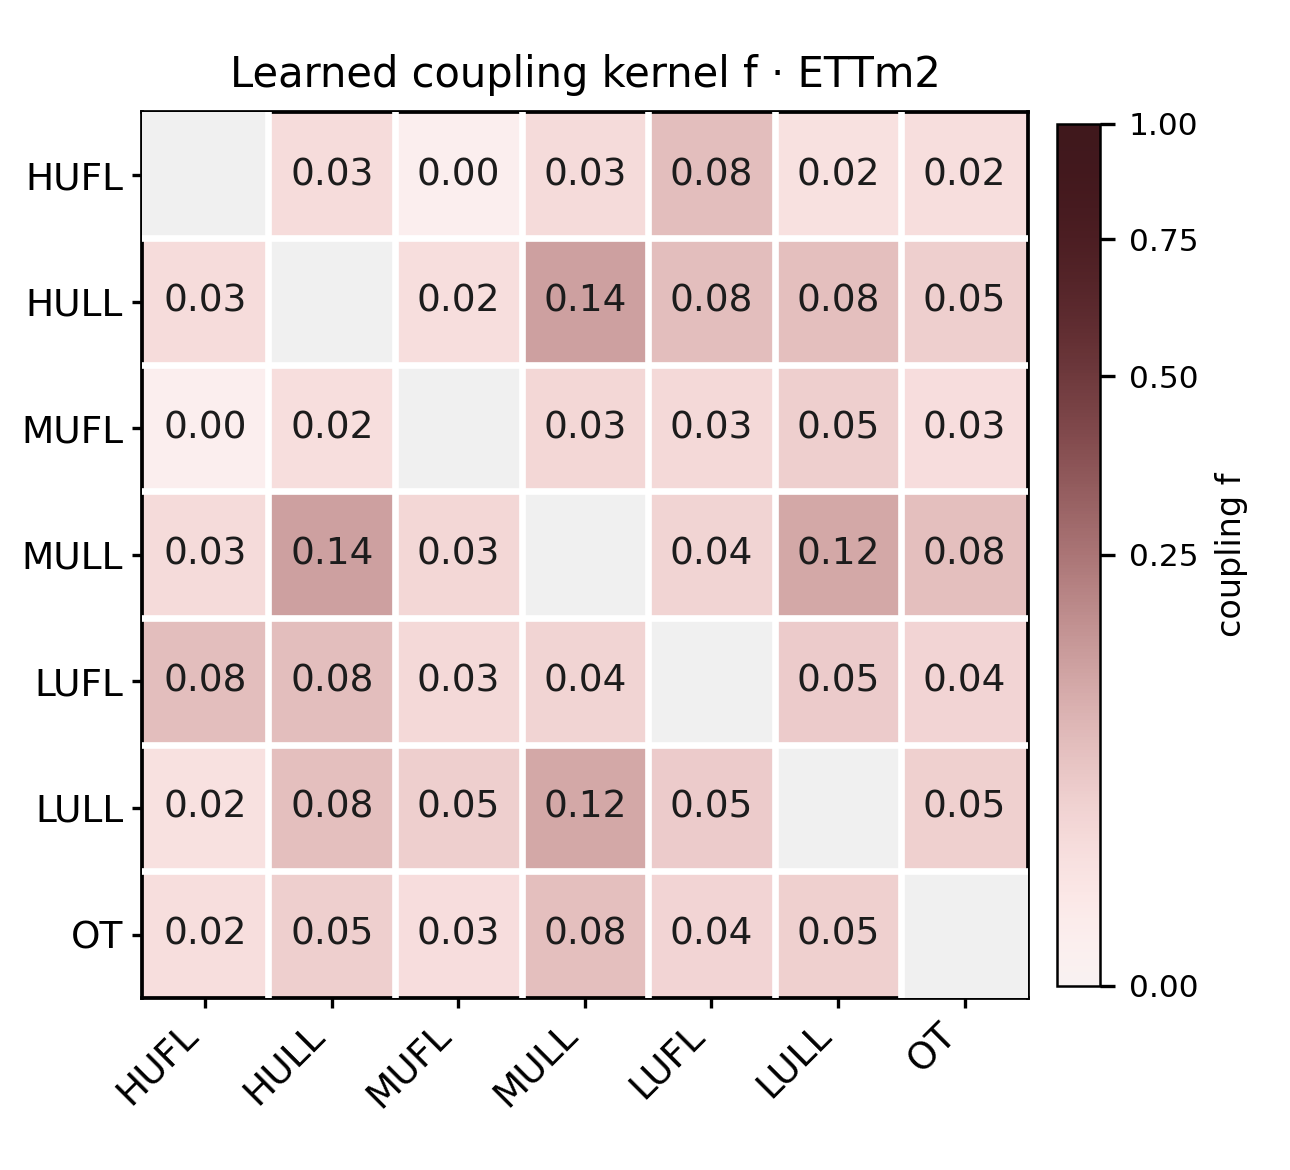
\includegraphics[width=0.475\textwidth]{ch5/figs/ch5_k_ETTm2.png}

\end{minipage}

\end{center}

\fi

ETTh1 的七个通道取自同一变电站：HUFL、HULL、MUFL、MULL、LUFL、LULL 分别是高压、中压、低压三个电压等级下的有用负荷与无用负荷，OT 为变压器油温。模型给出的耦合结构与这一物理分组吻合。
最强的一对是 HUFL 与 MUFL，耦合值 0.60，其次是 HULL 与 MULL，耦合值 0.31：前者是高压与中压的有用负荷，后者是高压与中压的无用负荷，即相邻电压层级上同类负荷之间的耦合最强。
相比之下，同一电压层级内有用负荷与无用负荷之间的耦合很弱，HUFL 与 HULL 只有 0.06，MUFL 与 MULL 只有 0.03，说明模型区分的是负荷的用途，而不是电压层级本身。
低压通道与其余通道普遍耦合很低，LUFL 与 LULL 各自与其余通道的平均耦合都在 0.03 以下，与低压侧负荷独立性强、对整站负荷驱动作用小一致。
油温 OT 与各负荷通道的耦合最弱，与其余通道的平均耦合只有 0.02，其中与 HULL 仅 0.01，这与油温是变压器负载的结果量、而非驱动量相符。
按通道看，与其余通道的平均耦合从高到低依次为高压与中压的有用负荷、高压与中压的无用负荷、低压负荷、油温，这一顺序与各通道在配电系统中的位置一致。

\ifchfivefigs

\begin{center}

\begin{minipage}{\textwidth}

\footnotesize

图 3d　ETTh1 在 720 步预测长度下的平均保真度核 f 非对角，用于比较不同预测长度下主要变量耦合关系。\\[2pt]

\centering

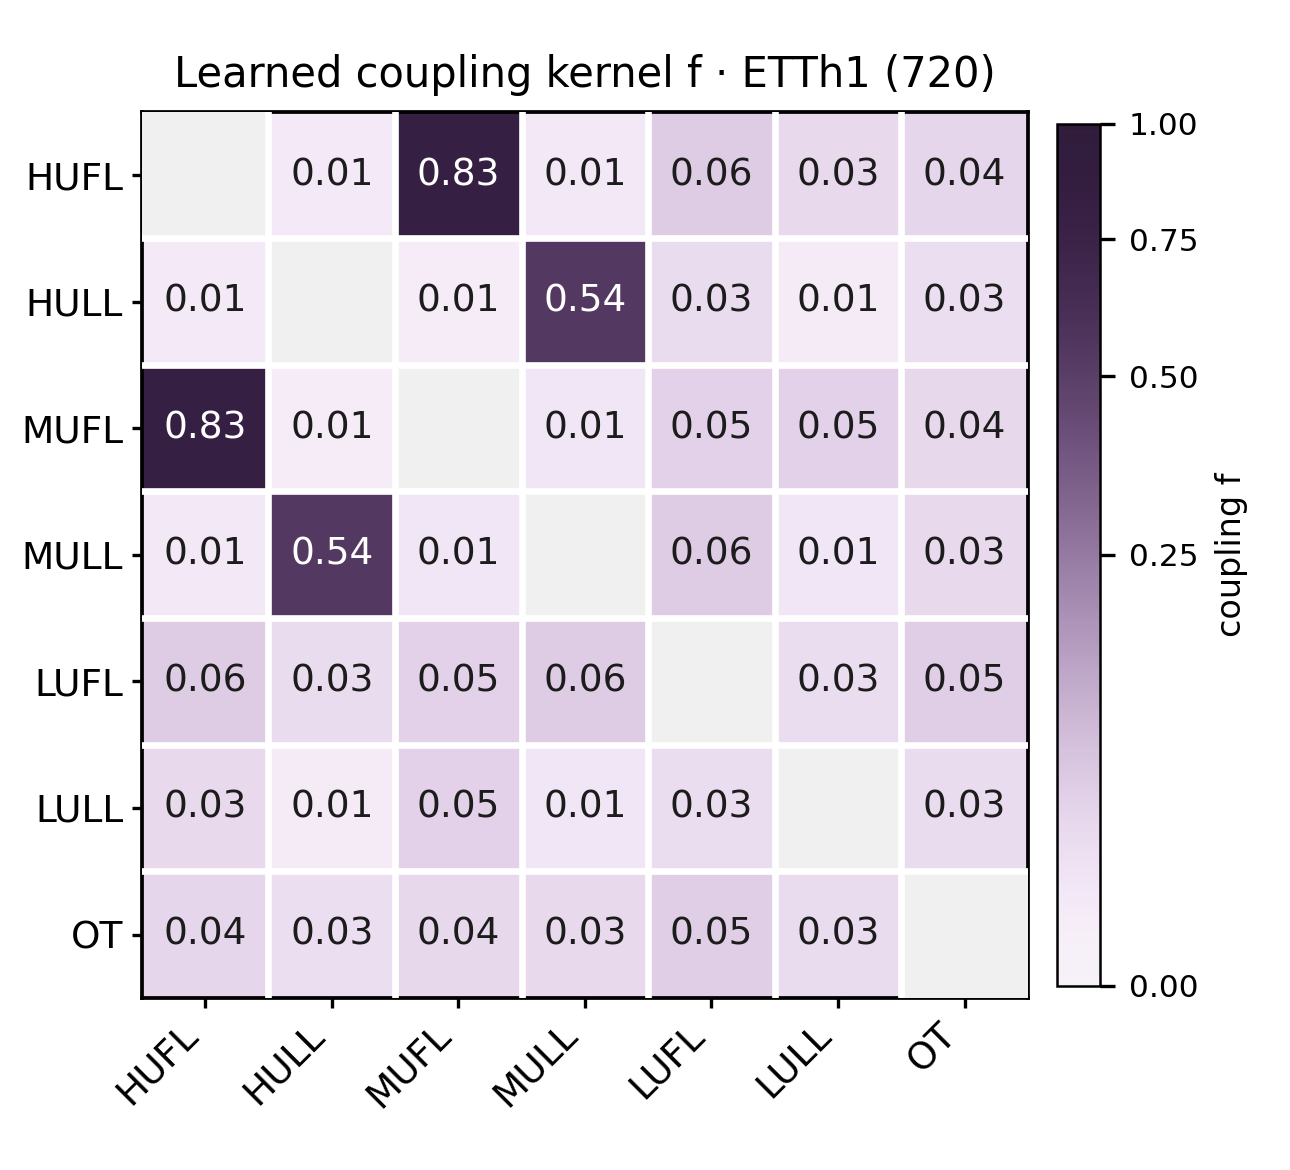
\includegraphics[width=0.475\textwidth]{ch5/figs/ch5_k_ETTh1_720.png}

\end{minipage}

\end{center}

\fi

不同数据集耦合分布的对比。
图 3c 用经验累计分布函数（Empirical Cumulative Distribution Function，ECDF）比较四类数据集非对角耦合值的分布：对每个数据集，我们收集平均 f 的全部非对角元素，纵轴给出不超过横轴对应耦合值的变量对比例。曲线在低值处快速上升，表示该数据集的耦合结构稀疏、绝大多数变量对耦合很弱；曲线整体更靠右，则表示存在更多强耦合对。
这里 ETTh1 与 ETTm2 上超过 0.1 的强对约占 10\%，而 ECL 与 Traffic 只约占 1\%，说明后者绝大多数变量对耦合微弱。该函数只用于描述不同数据集变量关系的稀疏与强弱，不用于声称预测性能。

\ifchfivefigs

\begin{center}

\begin{minipage}{\textwidth}

\footnotesize

图 3c　ETTh1、ETTm2、ECL 与 Traffic 非对角保真度核 f 值的经验累计分布函数（ECDF）：横轴为变量对的耦合强度 f，纵轴为不超过该值的变量对比例。\\[2pt]

\centering

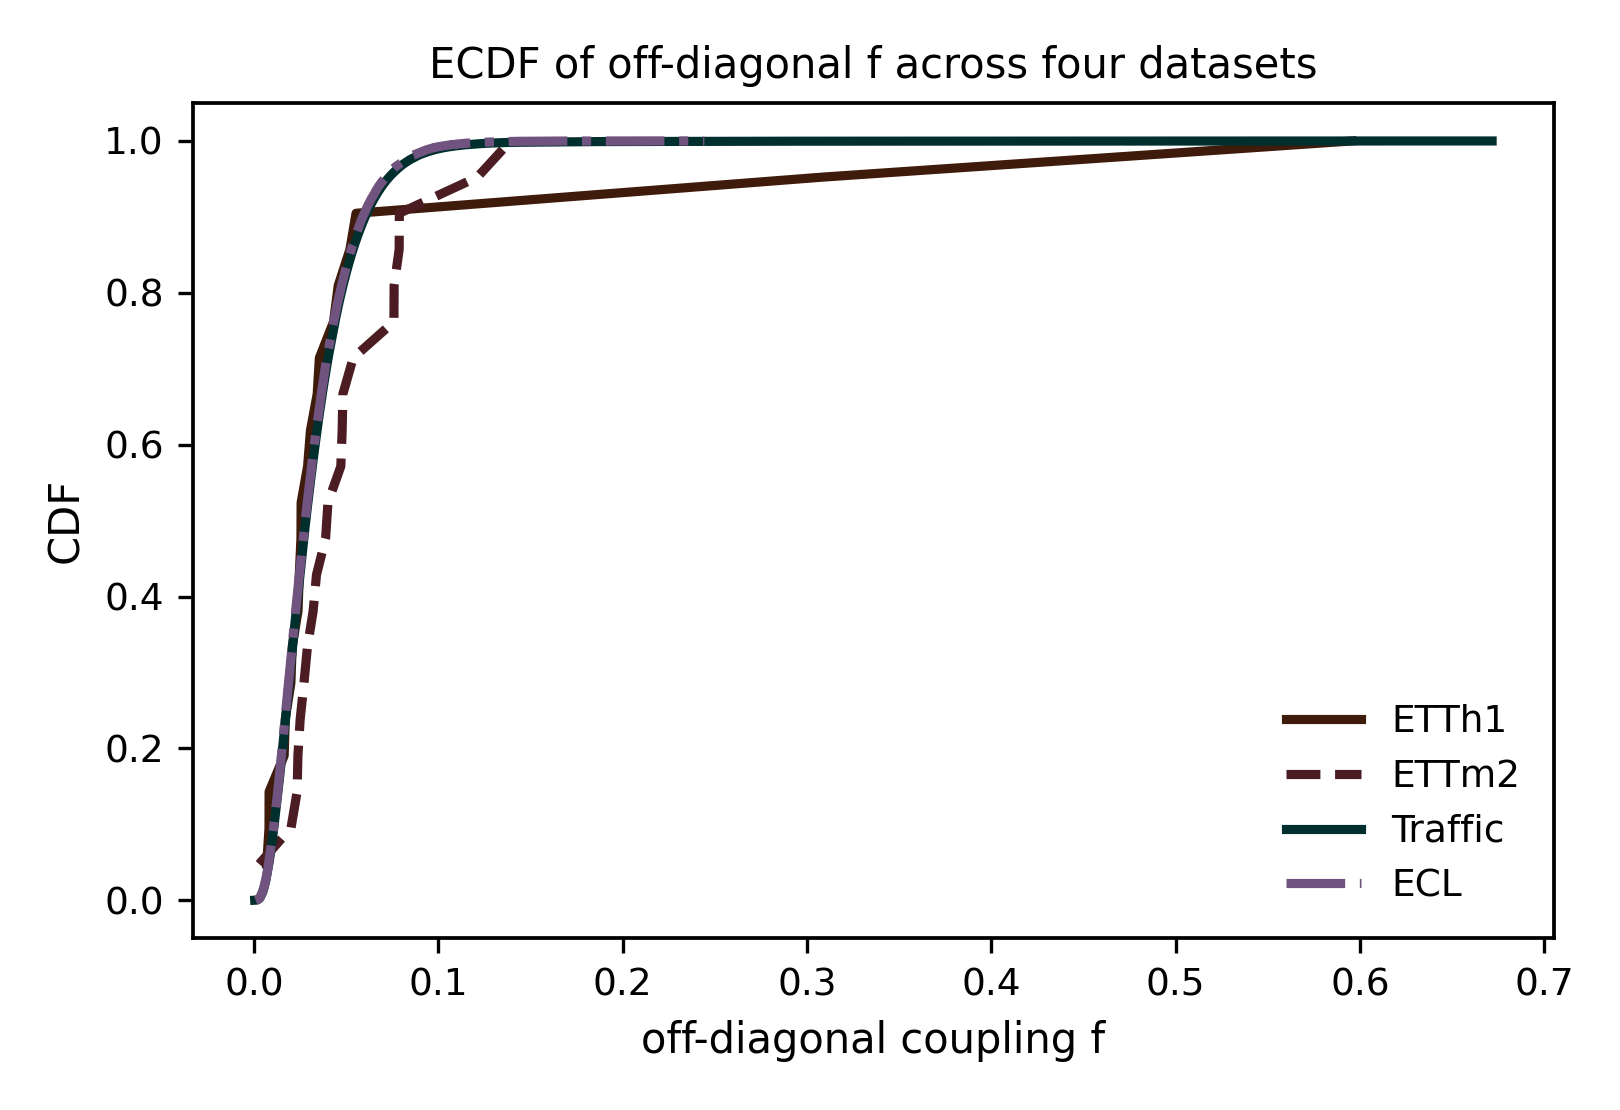
\includegraphics[width=0.656\textwidth]{ch5/figs/ch5_k_dist.png}

\end{minipage}

\end{center}

\fi

图 4 给出一个定性案例。在 ETTh1 的 96 步预测上，油温 OT 的真实曲线、基线主干与 QCCK-M 的预测如图所示：基线主干的预测整体偏低并在上升段明显滞后，QCCK-M 则更好地跟随了真值的走势，前 60 步的 MSE 由 0.0293 降到 0.0143。
这一案例与上文的耦合结构一致，耦合矩阵中读出的通道间强弱关系，在预测中体现为模型对不同通道的跟随能力。

\ifchfivefigs

\begin{center}

\begin{minipage}{\textwidth}

\footnotesize

图 4　ETTh1 在 96 步预测下 OT 通道的定性案例（真值、S-Mamba 与 QCCK-M）。\\[2pt]

\centering

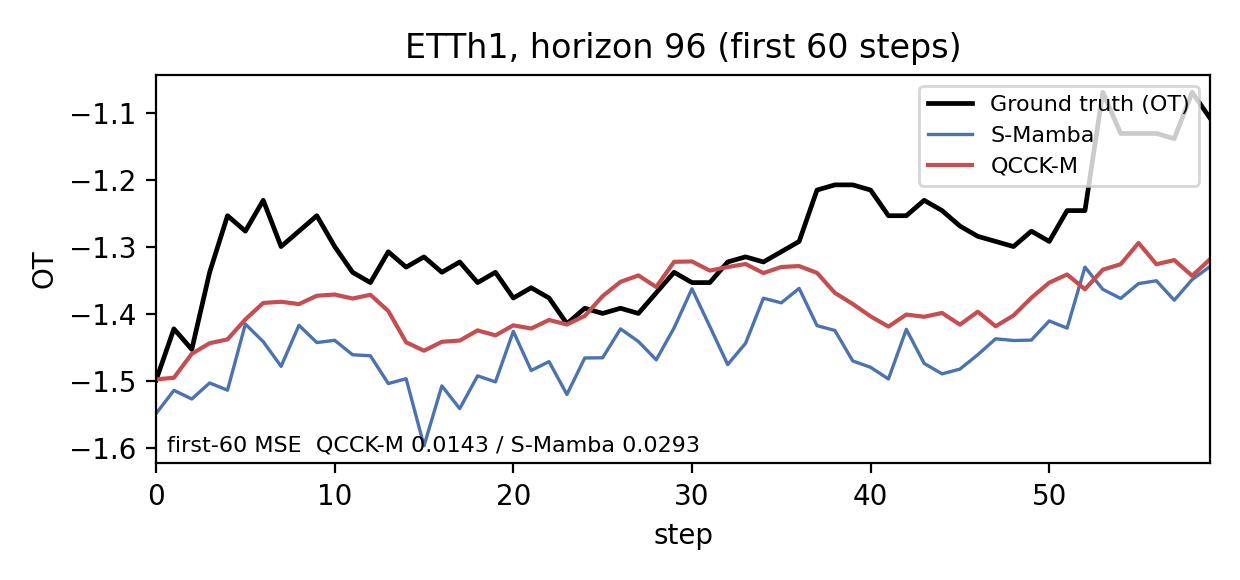
\includegraphics[width=0.812\textwidth]{ch5/figs/ch5_pred_ETTh1.png}

\end{minipage}

\end{center}

\fi

% [已移出] 参考文献块已挪到 references.tex（排在第六章结论之后），由 main.tex 统一 \input。
